\section{Języki pełnościeżkowe}

\begin{definicja}
	Język pełnościeżkowy to booleowska kombinacja języków postaci
	$$\mathrm{E}^{\textrm{liść}}L.$$
\end{definicja}

Sformułujemy teraz twierdzenie analogiczne do \ref{tw:sciezkowe}, charakteryzujące języki pełnościeżkowe poprzez ich algebrę syntaktyczną. Zauważmy najpierw, że twierdzenie w wersji dla języków ścieżkowych to rzeczywiście zbyt mało --- problematyczna jest tu równość $(ii)$: gdy za $g$ podstawimy pusty las otrzymamy:

$$v(0+h) = v0 + vh,$$

czyli

$$vh = v0 + vh.$$

Od razu widać, że ta równość niekoniecznie musi być spełniona, gdyż zbiór \textit{ścieżek liściowych} (pełnych ścieżek korzeń -- liść) prawej strony równości może być istotnie większy od zbioru pełnych ścieżek lewej strony.

Musimy więc nieco wzbogacić to twierdzenie, co uczynimy poniżej.

\begin{twierdzenie}
	Niech $L \subseteq H_A$ będzie regularnym językiem lasów. Niech $(H_L, V_L)$ będzie jego algebrą syntaktyczną. Następujące warunki są równoważne:
	
	\begin{enumerate}[(a)]
		\item $L$ jest językiem pełnościeżkowym
		\item $(H_L, V_L)$ spełnia:
		\begin{enumerate}[(i)]
			\item $h + g = g + h$ dla $h,g \in H_L$\label{(i)}
			\item $v(g+h) = vg + vh$ dla $v \in V_L$, $g,h \in H_L$, o ile $g,h$ są obrazami niepustych lasów\label{(ii)}
			\item $h + h = h$, dla $h \in H_L$.\label{(iii)}
		\end{enumerate}
	\end{enumerate}
\end{twierdzenie}

Poczyńmy kilka obserwacji:

\begin{fakt}
	Tak jak w przypadku języków ścieżkowych, równanie (\ref{(iii)}) jest konsekwencją równań (\ref{(i)}) oraz (\ref{(ii)}).
\end{fakt}

\begin{fakt}\label{fakt:homomorfizm}
	W odróżnieniu od języków ścieżkowych, rozstrzygnięcie czy dany język jest językiem pełnościeżkowym wymaga badania nie tylko algebry syntaktycznej, ale też homomorfizmu syntaktycznego.
\end{fakt}

Zatrzymajmy się na chwilę nad faktem \ref{fakt:homomorfizm}. Zauważmy, że modyfikacja twierdzenia \ref{tw:sciezkowe} polegała na dodaniu do równości (\ref{(ii)}) założenia ,,o ile $g,h$ są obrazami niepustych lasów''. Rzeczywiście opisuje to homomorfizm, a nie algebrę. Aby zilustrować ten fakt, przyjrzyjmy się następującemu przykładowi.

\begin{przyklad}
	Przedstawimy dwa języki spośród których tylko jeden jest językiem pełnościeżkowym. Oba za to mają taką samą algebrę syntaktyczną.
	
	\begin{itemize}
		\item $L = \textrm{,,istnieje liść $a$''},$ $A = \{a,b\}$,
		\item $L' = \textrm{,,po usunięciu $c$ istnieje liść $a$''},$ $A = \{a,b,c\}$.
	\end{itemize}
	
	Przez ,,usunięcie $c$'' rozumiemy następującą operację:
	
	\begin{center}
		\begin{minipage}[t]{.25\linewidth}
			\vspace{0pt}
			\centering
			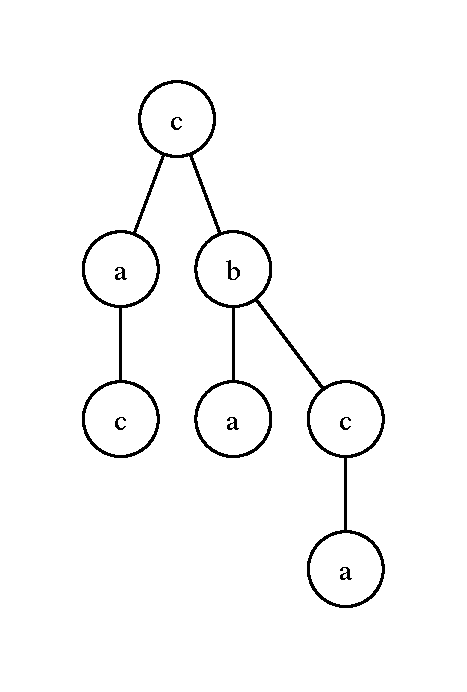
\includegraphics[scale=0.6]{rysunki/w12-usuniecie_c_1.pdf}
		\end{minipage}
		\begin{minipage}[t]{.25\linewidth}
			\centering 
			\vspace{40pt}
			\begin{displaymath}
				\xymatrix{ 
					\ar@{~>}[rr]^{\textrm{usunięcie $c$}} &&
				}
			\end{displaymath}
		\end{minipage}
		\begin{minipage}[t]{.25\linewidth}
			\vspace{0pt}
			\centering
			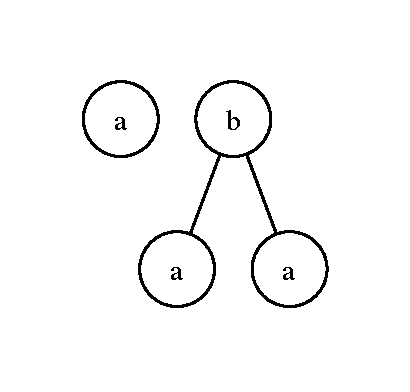
\includegraphics[scale=0.6]{rysunki/w12-usuniecie_c_2.pdf}
		\end{minipage}
	\end{center}
	
	Oczywiście $L$ jest językiem pełnościeżkowym. Oba te języki mają taką samą algebrę syntaktyczną --- danemu $t' \in L'$ przypisany jest ten sam element algebry co odpowiadającemu mu $t \in L$ (tzn. osiągniętemu przez usunięcie $c$).
	
	$L'$ nie jest za to językiem pełnościeżkowym. Rozpatrzmy przedstawione poniżej lasy $t_1$ (po lewej) oraz $t_2$. Odpowiadający im zbiór ścieżek liściowych jest taki sam (a więc jest im przyporządkowany ten sam element algebry syntaktycznej), ale $t_1 \in L'$, a $t_2 \notin L'$.
	
	\begin{center}
		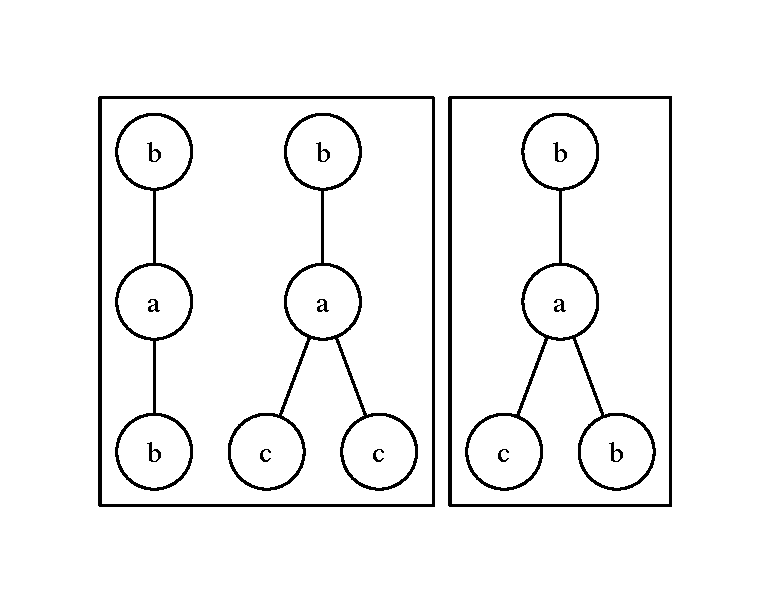
\includegraphics[scale=0.6]{rysunki/w12-l_prim.pdf}
	\end{center}
	
\end{przyklad}